\begin{centering}
    \subsection{Сравнение тестов проверки условной независимости}\label{numerical_exp}
\end{centering}
Кратко напомним тесты, которые будут сравниваться.
\begin{enumerate}
    \item $\varphi^{\text{Theta}}$ -- РНМН тест уровня 
    $\alpha=0.05$ для проверки гипотезы 
     $$\theta := \ln  \left(\dfrac{p_{001}p_{111}p_{010}p_{100}}{p_{011}p_{101}p_{000}p_{110}}\right)=0$$
    Поскольку из $X \ci Y \mid Z$ следует $\theta=0$, 
    то $\varphi^{\text{Theta}}$ является тестом уровня $\alpha=0.05$ для проверки
    гипотезы $h:X \ci Y \mid Z$.
    \item $\varphi^{\text{Subsamples}}$ -- тест уровня $\alpha=0.05$
    для проверки $h: X \ci Y \mid Z$.
    Гипотеза $h$ отвергается, если РНМН-тестами уровня 
    $\gamma=1-\sqrt{1-\alpha}$
    отвергается хотя бы 
    одна гипотеза 
    $\theta_z := \ln\left(\dfrac{p_{00z}p_{11z}}{p_{01z}p_{10z}}\right)=0$
    по подвыборке из условного распределения $(X,Y)^T$ при условии $Z=z$.
    \item $\varphi^{\text{Partial}}$ -- точный тест уровня $\alpha=0.05$
    для проверки гипотезы $\rho^{XY\cdot Z}=0$ в трехмерном нормальном распределении.
    Если $\varphi^{\text{Partial}}$ -- также тест
    уровня $\alpha=0.05$ для проверки гипотезы $\rho^{XY\cdot Z}=0$ в трехмерном распределении Бернулли, 
    то $\varphi^{\text{Partial}}$ -- тест уровня $\alpha=0.05$ для проверки
    гипотезы $h:X \ci Y \mid Z$ в трехмерном распределении Бернулли,
    поскольку из $X \ci Y \mid Z$ следует $\rho^{XY\cdot Z}=0$.
\end{enumerate}

\begin{figure}[H]
    \centering
    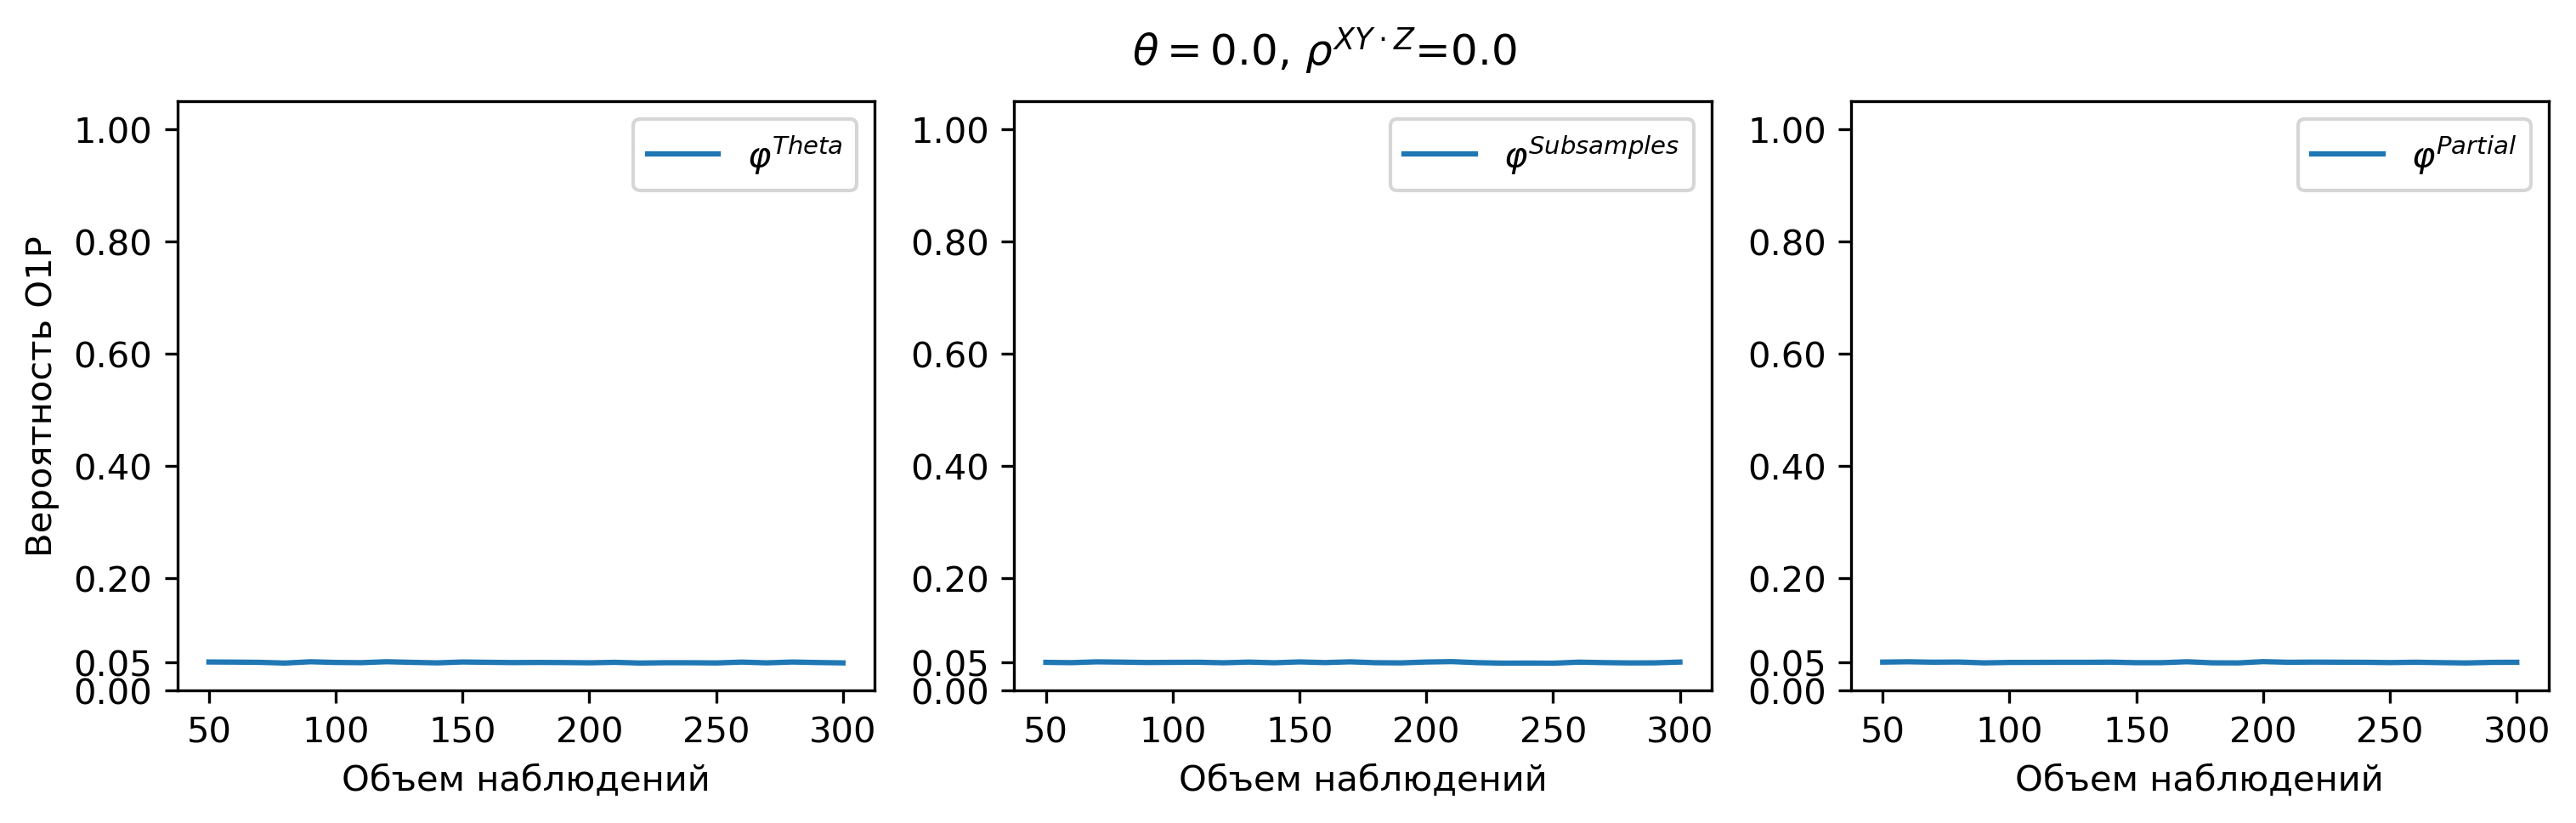
\includegraphics[scale=0.55]{images/graph1.png}
    \caption{Графики зависимости вероятности ошибки 1 рода (О1Р) от количества наблюдений
    на тестах $\varphi^{\text{Theta}}$, $\varphi^{\text{Subsamples}}$, $\varphi^{\text{Partial}}$
    в трехмерном распределении Бернулли с $p_{000}=0.125, p_{001}=0.125, p_{010}=0.125, p_{011}=0.125,
    p_{100}=0.125, p_{101}=0.125, p_{110}=0.125, p_{111}=0.125$. 
    Гипотеза $h: X \ci Y \mid Z$ верна.
    Вероятности оцениваются по $10^5$ экспериментам.} \label{fig:1}
\end{figure}
    

\begin{figure}[H]
    \centering
    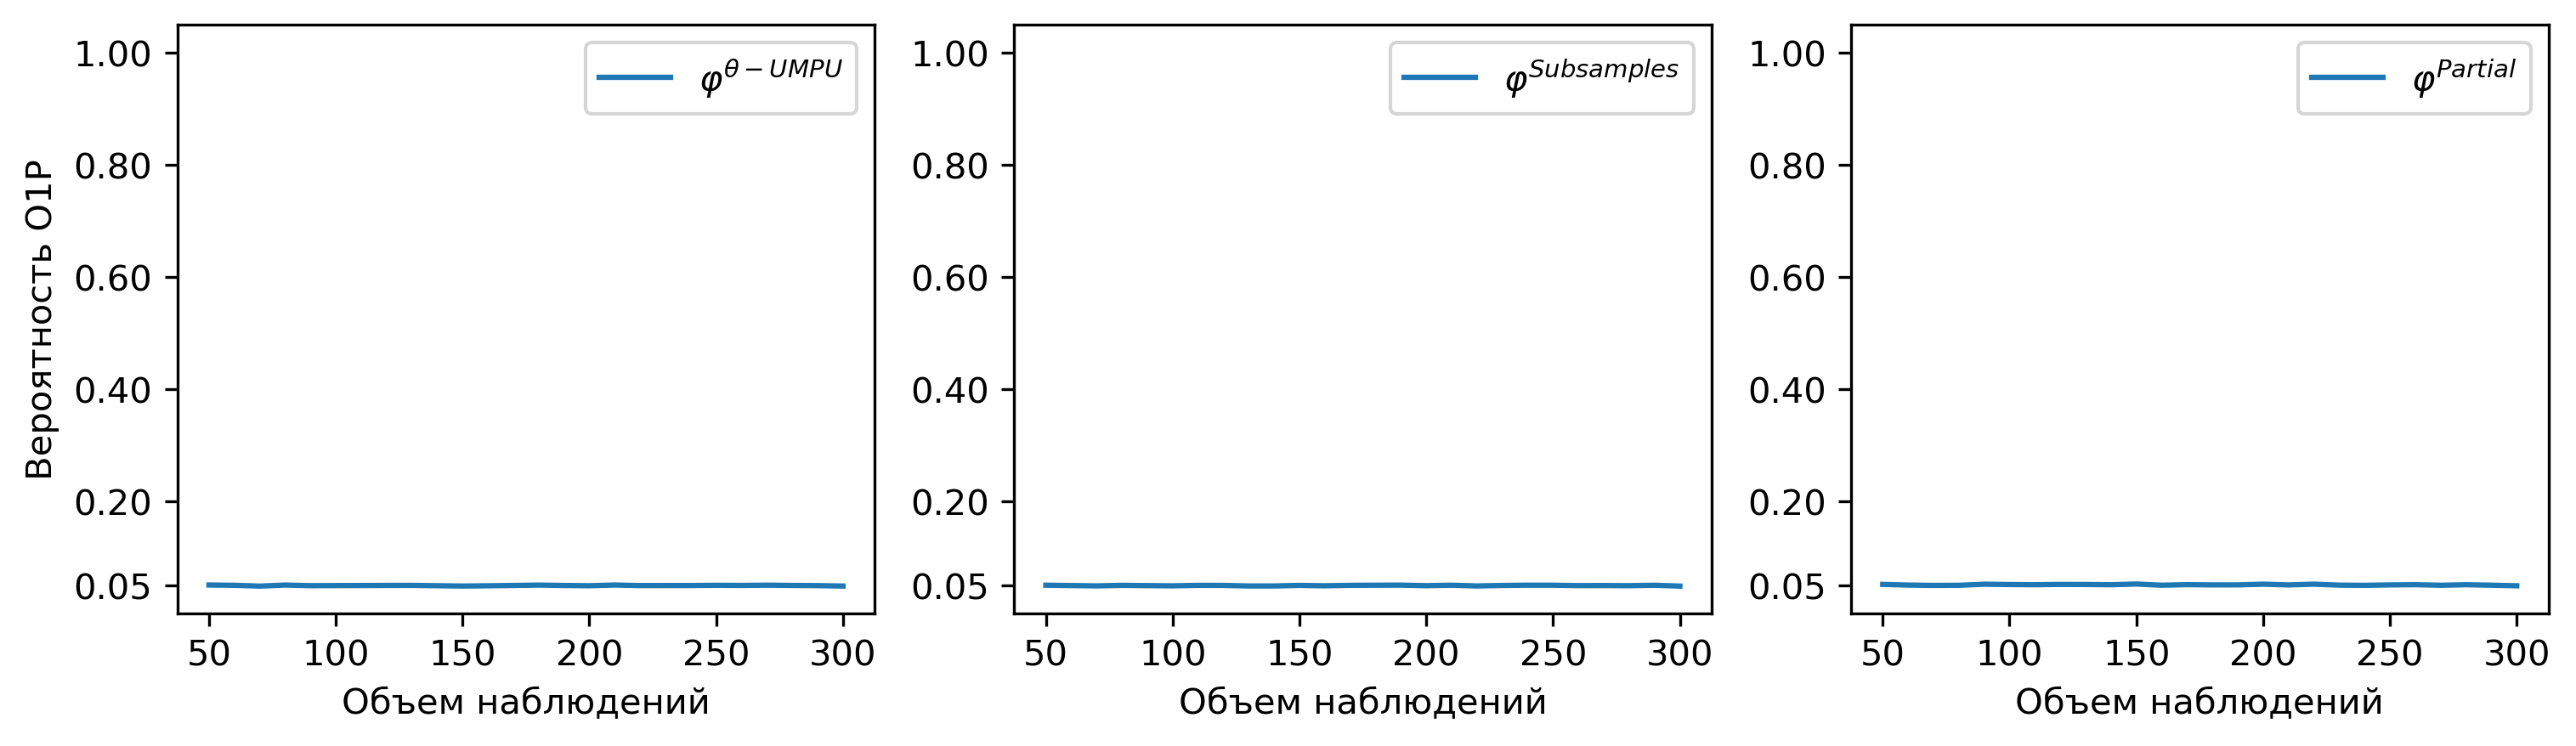
\includegraphics[scale=0.55]{images/graph2.png}
    \caption{Графики зависимости вероятности ошибки 1 рода (О1Р) от количества наблюдений
    на тестах $\varphi^{\text{Theta}}$, $\varphi^{\text{Subsamples}}$, $\varphi^{\text{Partial}}$
    в трехмерном распределении Бернулли с $p_{000}=0.15, p_{001}=0.1, p_{010}=0.3, p_{011}=0.1,
    p_{100}=0.05, p_{101}=0.1, p_{110}=0.1, p_{111}=0.1$. 
    Гипотеза $h: X \ci Y \mid Z$ верна.
    Вероятности оцениваются по $10^5$ экспериментам.} \label{fig:2}
\end{figure}

Из (\autoref{fig:1}) и (\autoref{fig:2}) видно, что тесты $\varphi^{\text{Theta}}$, $\varphi^{\text{Subsamples}}$, 
$\varphi^{\text{Partial}}$ контролируют вероятность 
ошибки первого рода на уровне $\alpha=0.05$. Для тестов $\varphi^{\text{Theta}}$, $\varphi^{\text{Subsamples}}$
данный результат согласуется с теорией.
Неожиданным оказывается факт того,
что тест $\varphi^{\text{Partial}}$ контролирует вероятность
ошибки первого рода на уровене $\alpha=0.05$ в трехмерном
распределении Бернулли, хотя данный тест теоретически обоснован только для трехмерного нормального 
распределения.

\begin{figure}[H]
    \centering
    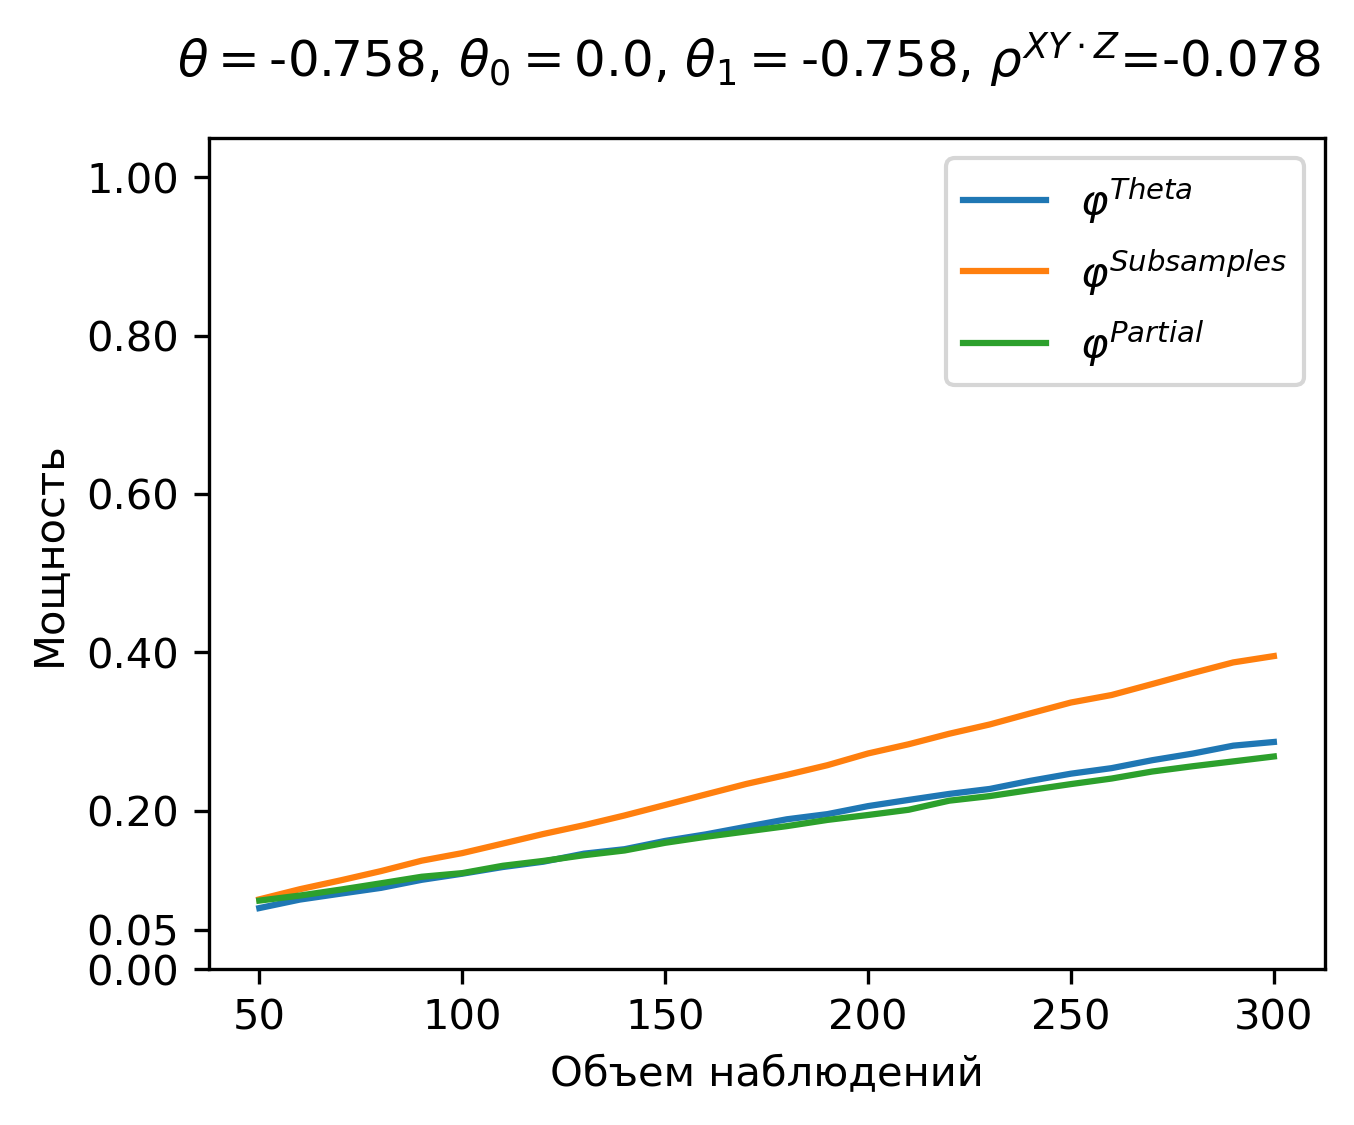
\includegraphics[scale=0.6]{images/graph3.png}
    \caption{График зависимости мощности от количества наблюдений
    на тестах $\varphi^{\text{Theta}}$, $\varphi^{\text{Subsamples}}$, $\varphi^{\text{Partial}}$
    в трехмерном распределении Бернулли с $p_{000}=0.15, p_{001}=0.06, 
    p_{010}=0.3, p_{011}=0.16,
    p_{100}=0.05, p_{101}=0.08, p_{110}=0.1, p_{111}=0.1$. 
    Гипотеза $h: X \ci Y \mid Z$ не верна, однако $X$ и $Y$ независимы
    при условии $Z=0$, 
    Мощность оцениваются по $10^5$ экспериментам.}\label{fig:3}
\end{figure}

Одним из возможных отклонений от условной независимости является случай,
когда $X$ и $Y$ независимы при условии $Z=0$, но зависимы при условии $Z=1$.
Такой случай представлен на (\autoref{fig:3}), в нём даже при $n=300$ наблюдениях все тесты показывают
низкую мощность.

\begin{figure}[H]
    \centering
    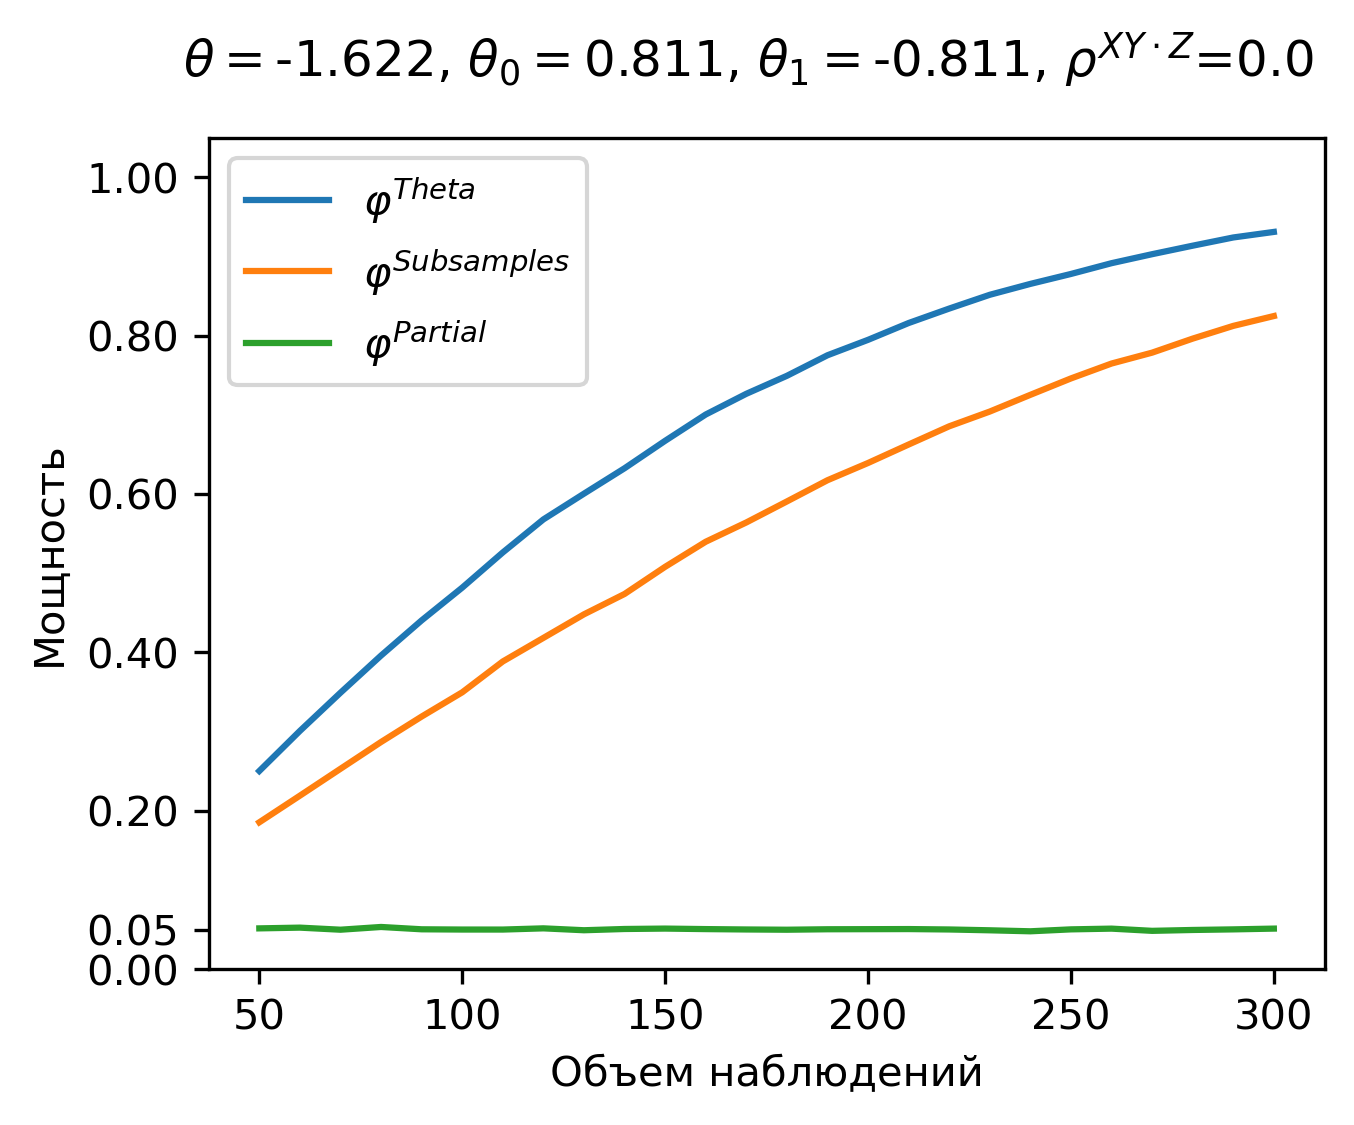
\includegraphics[scale=0.6]{images/graph4.png}
    \caption{График зависимости мощности от количества наблюдений
    на тестах $\varphi^{\text{Theta}}$, $\varphi^{\text{Subsamples}}$, $\varphi^{\text{Partial}}$
    в трехмерном распределении Бернулли с $p_{000}=0.15, p_{001}=0.1, 
    p_{010}=0.1, p_{011}=0.15,
    p_{100}=0.1, p_{101}=0.15, p_{110}=0.15, p_{111}=0.1$. 
    Гипотеза $h: X \ci Y \mid Z$ не верна, однако верна гипотеза $\rho^{XY\cdot Z}=0$.
    Вероятности оцениваются по $10^5$ экспериментам.} \label{fig:4}
\end{figure}

\begin{figure}[H]
    \centering
    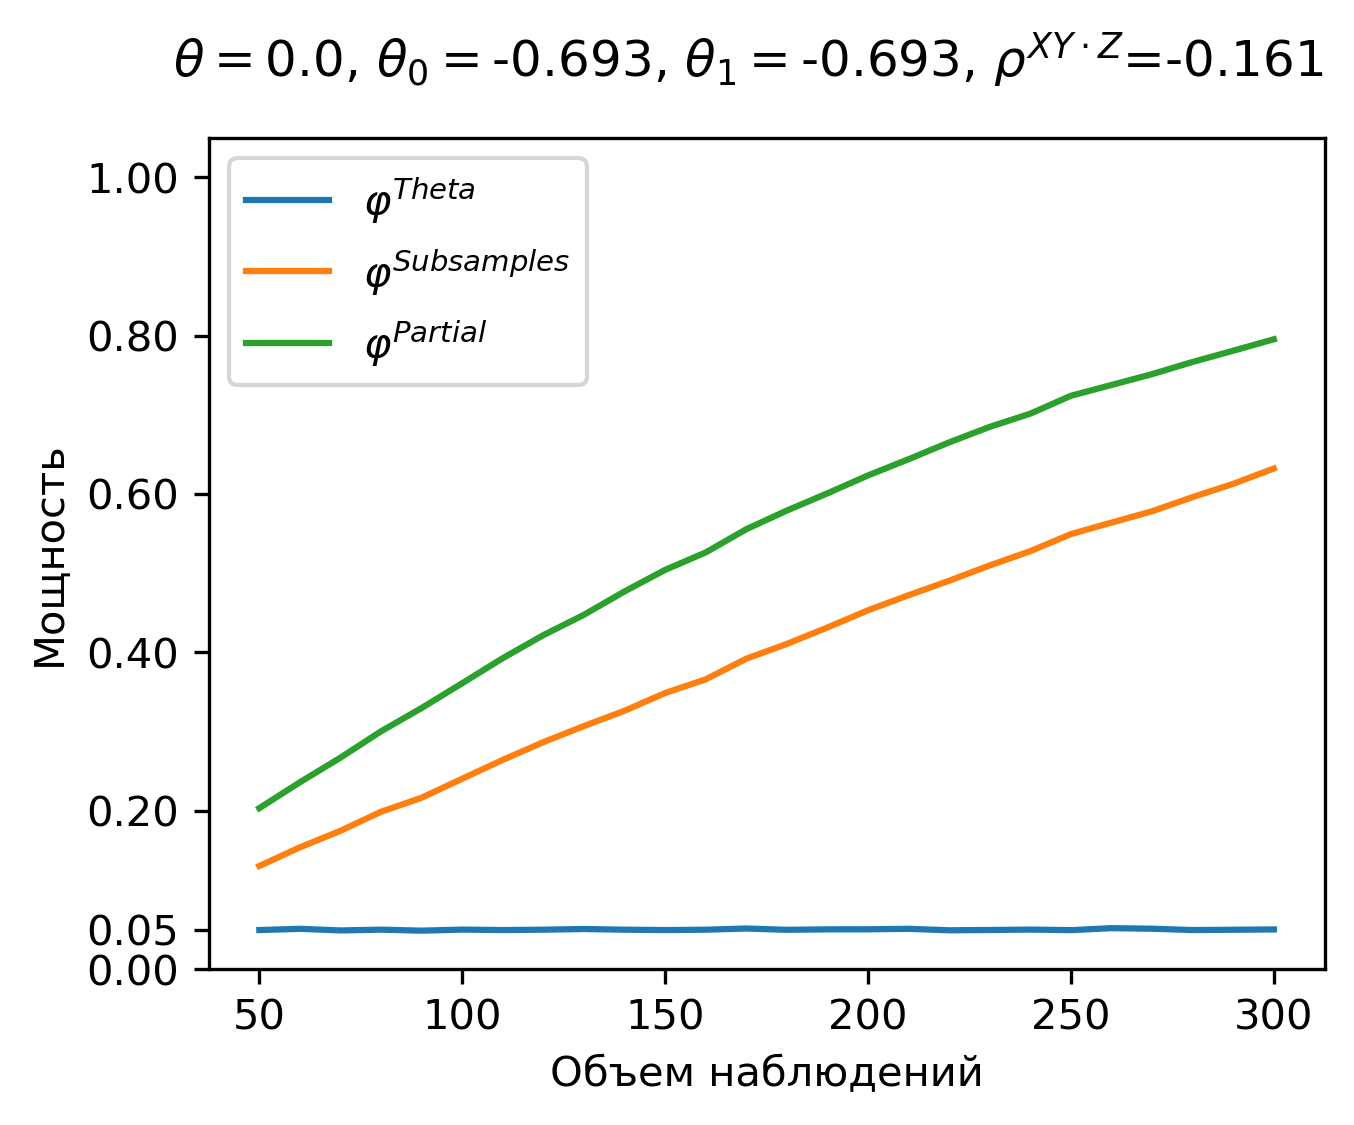
\includegraphics[scale=0.6]{images/graph5.png}
    \caption{График зависимости мощности от количества наблюдений
    на тестах $\varphi^{\text{Theta}}$, $\varphi^{\text{Subsamples}}$, $\varphi^{\text{Partial}}$
    в трехмерном распределении Бернулли с $p_{000}=0.15, p_{001}=0.05, 
    p_{010}=0.3, p_{011}=0.1,
    p_{100}=0.1, p_{101}=0.1, p_{110}=0.1, p_{111}=0.1$. 
    Гипотеза $h: X \ci Y \mid Z$ не верна, однако верна гипотеза $\theta=0$.
    Вероятности оцениваются по $10^5$ экспериментам.} \label{fig:5}
\end{figure}

Графики (\autoref{fig:4}) и (\autoref{fig:5}) показывают, что тесты 
$\varphi^{\text{Theta}}$, $\varphi^{\text{Subsamples}}$
проверяют бóльшие гипотезы чем $h: X \ci Y \mid Z$.
В частности, на (\autoref{fig:4}) и (\autoref{fig:5})
параметры $\rho^{XY\cdot Z}=0$ и $\theta=0$ соответственно, но гипотеза
$h: X \ci Y \mid Z$ не верна.

\begin{figure}[H]
    \centering
    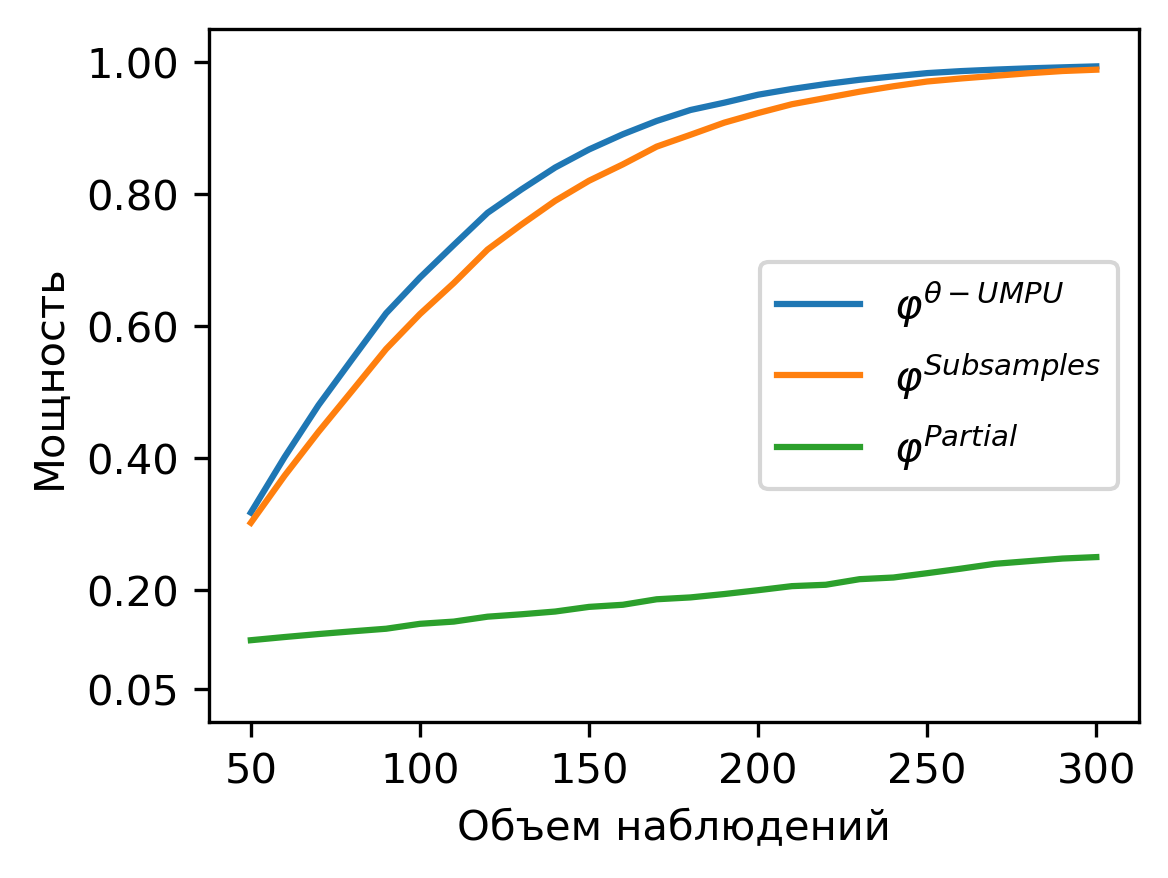
\includegraphics[scale=0.6]{images/graph6.png}
    \caption{График зависимости мощности от количества наблюдений
    на тестах $\varphi^{\text{Theta}}$, $\varphi^{\text{Subsamples}}$, $\varphi^{\text{Partial}}$
    в трехмерном распределении Бернулли с $p_{000}=0.03, p_{001}=0.1, 
    p_{010}=0.04, p_{011}=0.08,
    p_{100}=0.3, p_{101}=0.1, p_{110}=0.07, p_{111}=0.28$. 
    Гипотеза $h: X \ci Y \mid Z$ не верна.
    Вероятности оцениваются по $10^5$ экспериментам.} \label{fig:6}
\end{figure}

Показательным является пример с (\autoref{fig:6}). Тесты 
$\varphi^{\text{Theta}}$ и $\varphi^{\text{Subsamples}}$ при $n=300$
наблюдениях имеют мощность, близкую к $1$. В то время как мощность
теста $\varphi^{\text{Partial}}$ приблизительно равна $0.25$. Это происходит потому, что
в данном примере значение $\rho^{XY\cdot Z}=0.068$ близко к нулю.

\begin{figure}[H]
    \centering
    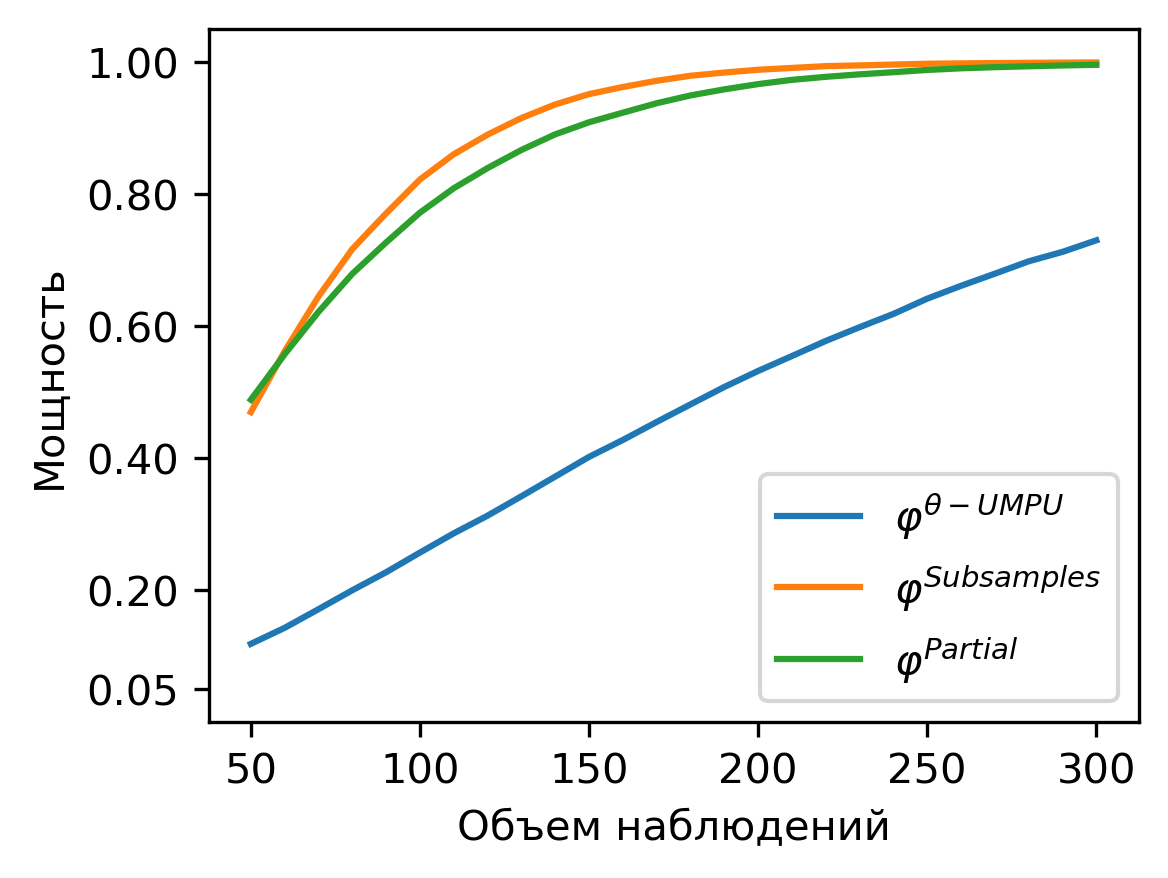
\includegraphics[scale=0.6]{images/graph7.png}
    \caption{График зависимости мощности от количества наблюдений
    на тестах $\varphi^{\text{Theta}}$, $\varphi^{\text{Subsamples}}$, $\varphi^{\text{Partial}}$
    в трехмерном распределении Бернулли с $p_{000}=0.21, p_{001}=0.12, 
    p_{010}=0.04, p_{011}=0.34,
    p_{100}=0.1, p_{101}=0.12, p_{110}=0.02, p_{111}=0.05$. 
    Гипотеза $h: X \ci Y \mid Z$ не верна.
    Вероятности оцениваются по $10^5$ экспериментам.} \label{fig:7}
\end{figure}

Еще интересен пример с (\autoref{fig:7}). 
При $n=300$ наблюдениях мощность тестов
$\varphi^{\text{Subsamples}}$, $\varphi^{\text{Partial}}$ близка к $1$,
в то время как мощность теста $\varphi^{\text{Theta}}$ примерно равна $0.73$.

В данном разделе были изложены результаты численных экспериментов с тестами
$\varphi^{\text{Theta}}$, $\varphi^{\text{Subsamples}}$, 
$\varphi^{\text{Partial}}$ при $\alpha=0.05$. На 
(\autoref{fig:1}) и (\autoref{fig:2}) показано, что 
при истинности гипотезы  
$h: X \ci Y \mid Z$ эти тесты контролируют вероятность ошибки первого рода
на уровне $\alpha=0.05$. 
Однако, за счет того, что тесты 
$\varphi^{\text{Subsamples}}$ и
$\varphi^{\text{Partial}}$ проверяют более широкие гипотезы,
возникают ситуации как на 
 (\autoref{fig:4}) и (\autoref{fig:5}), когда гипотеза $h: X \ci Y \mid Z$
не верна и мощность теста равна $0.05$ при любом объеме наблюдений.
Особым образом можно выделить тест $\varphi^{\text{Subsamples}}$.
На всех графиках $\varphi^{\text{Subsamples}}$ либо лучший по мощности,
либо незначительно уступает лучшему по мощности тесту.
